\chapter{Kết quả thực nghiệm}
\ifpdf
\graphicspath{{Chapter4/Chapter4Figs/PNG/}{Chapter4/Chapter4Figs/PDF/}{Chapter4/Chapter4Figs/}}
\else
\graphicspath{{Chapter4/Chapter4Figs/EPS/}{Chapter4/Chapter4Figs/}}
\fi
\begin{quote}
	\textit{Trong chương này, chúng em trình bày kết quả thực nghiệm của bài toán tự động chơi game.
	Đầu tiên, môi trường giả lập của bài toán tự động chơi game cùng với các thiết lập thực nghiệm được giới thiệu.
	Phần tiếp theo, chúng em trình bày về kết quả thực nghiệm của thuật toán ``Q-learning'' để chứng minh tính khả thi của việc kết hợp học tăng cường với học sâu vào bài toán tự động chơi game.
	Kế tiếp, chúng em phân tích mức độ ảnh hưởng của vấn đề ``đánh giá quá cao'' và kết quả của thuật toán ``Double Q-learning''.
	Phần cuối cùng bao gồm một số thực nghiệm chứng minh rằng mô hình mạng nơ-ron xấp xỉ tốt hàm giá trị hành động.}
\end{quote}
 
\section{Giới thiệu Arcade Learning Environment}
Arcade Learning Environment (ALE) là một framework được thiết kế giúp dễ dàng trong việc phát triển những hệ thống có thể tự động chơi bất kỳ những game trên hệ máy Atari 2600.
\subsection{Hệ máy Atari 2600}
\ref{fig:AtariConsole} là hệ máy chơi game Atari 2600 tại gia đình được phát triển và sử dụng phổ biến vào những năm 1970.
Hơn 500 game đã được phát triển cho hệ máy này; một số game vẫn tiếp tục được phát triển cho tới ngày nay. 
Độ phân giải của những game này là $210 \times 160$. 
Mặc dù vậy nhiều game được phát triển cho hệ máy này, nhưng cấu hình phần cứng của chúng khá đơn giản bao gồm một CPU 1.19 Mhz, một bộ nhớ ROM 2-4KB để lưu giữ code của game, và dung lượng RAM của máy cũng chỉ là 128 bytes. 
Đồ họa của các game được cố định ở độ phân giải $160 x 210$, với ảnh màu RGB. 
Người chơi tương tác với game qua một thiết bị được gọi là joystick, có thể thực hiện tối đa 18 hành động.

\subsection{Interface}
ALE được xây dựng trên nền Stella, nó giả lập máy hệ máy Atari 2600. Qua đó cho phép người dùng tương tác với Atari 2600 bằng cách tiếp nhận những di chuyển của joystick, gửi thông tin của game cho người dùng như hình ảnh, điểm số nhận được. 
ALE cũng cung cấp một \textit{lớp sử lý} để chuyển đổi những thông tin trong game theo chuẩn của bài toán học tăng cường như điểm số đạt được, kết thúc game chưa. 
Mặc định, lớp này biểu diễn mỗi trạng thái trong game bằng một mảng 7-bit pixels 2 chiều, và không gian hành động gồm 18 hành động tương ứng với các hành động có thể thực hiện trong joystick. 
Lớp sử lý cung cấp thông tin tập những hành động cụ thể có thể thực hiện trong một game. 
ALE có thể tạo ra 60 frame hình ảnh game trong một giây theo mặc định, và số frame ảnh nhiều nhất trong một giây nó có thể tạo ra 6000 frame. 
Điểm số nhận được tại từng thời điểm được định nghĩa theo từng game khác nhau. 
Một mẫu thực nghiệm có thể được tao ra từ frame đầu tiên của game cho đến khi game kết thúc, ngoài ra lớp sử lý cũng cho phép người người tạo mãu thực nghiệm với số lượng frame cố định.

ALE hơn nữa cũng cung cấp chức năng \textit{sao lưu} và \textit{khôi phục} trạng thái của game. 
Khi lệnh sao lưu được thực thi, ALE lưu lại tất cả các dữ liệu liên quan tại thời điểm đó trong game như nội dung RAM, registers. 
Ngược lại khi lệnh khôi phục được thực thi, nó sẽ khởi tạo lại trạng thái game đã lưu lại trước đó.

\begin{figure}
	\centering
	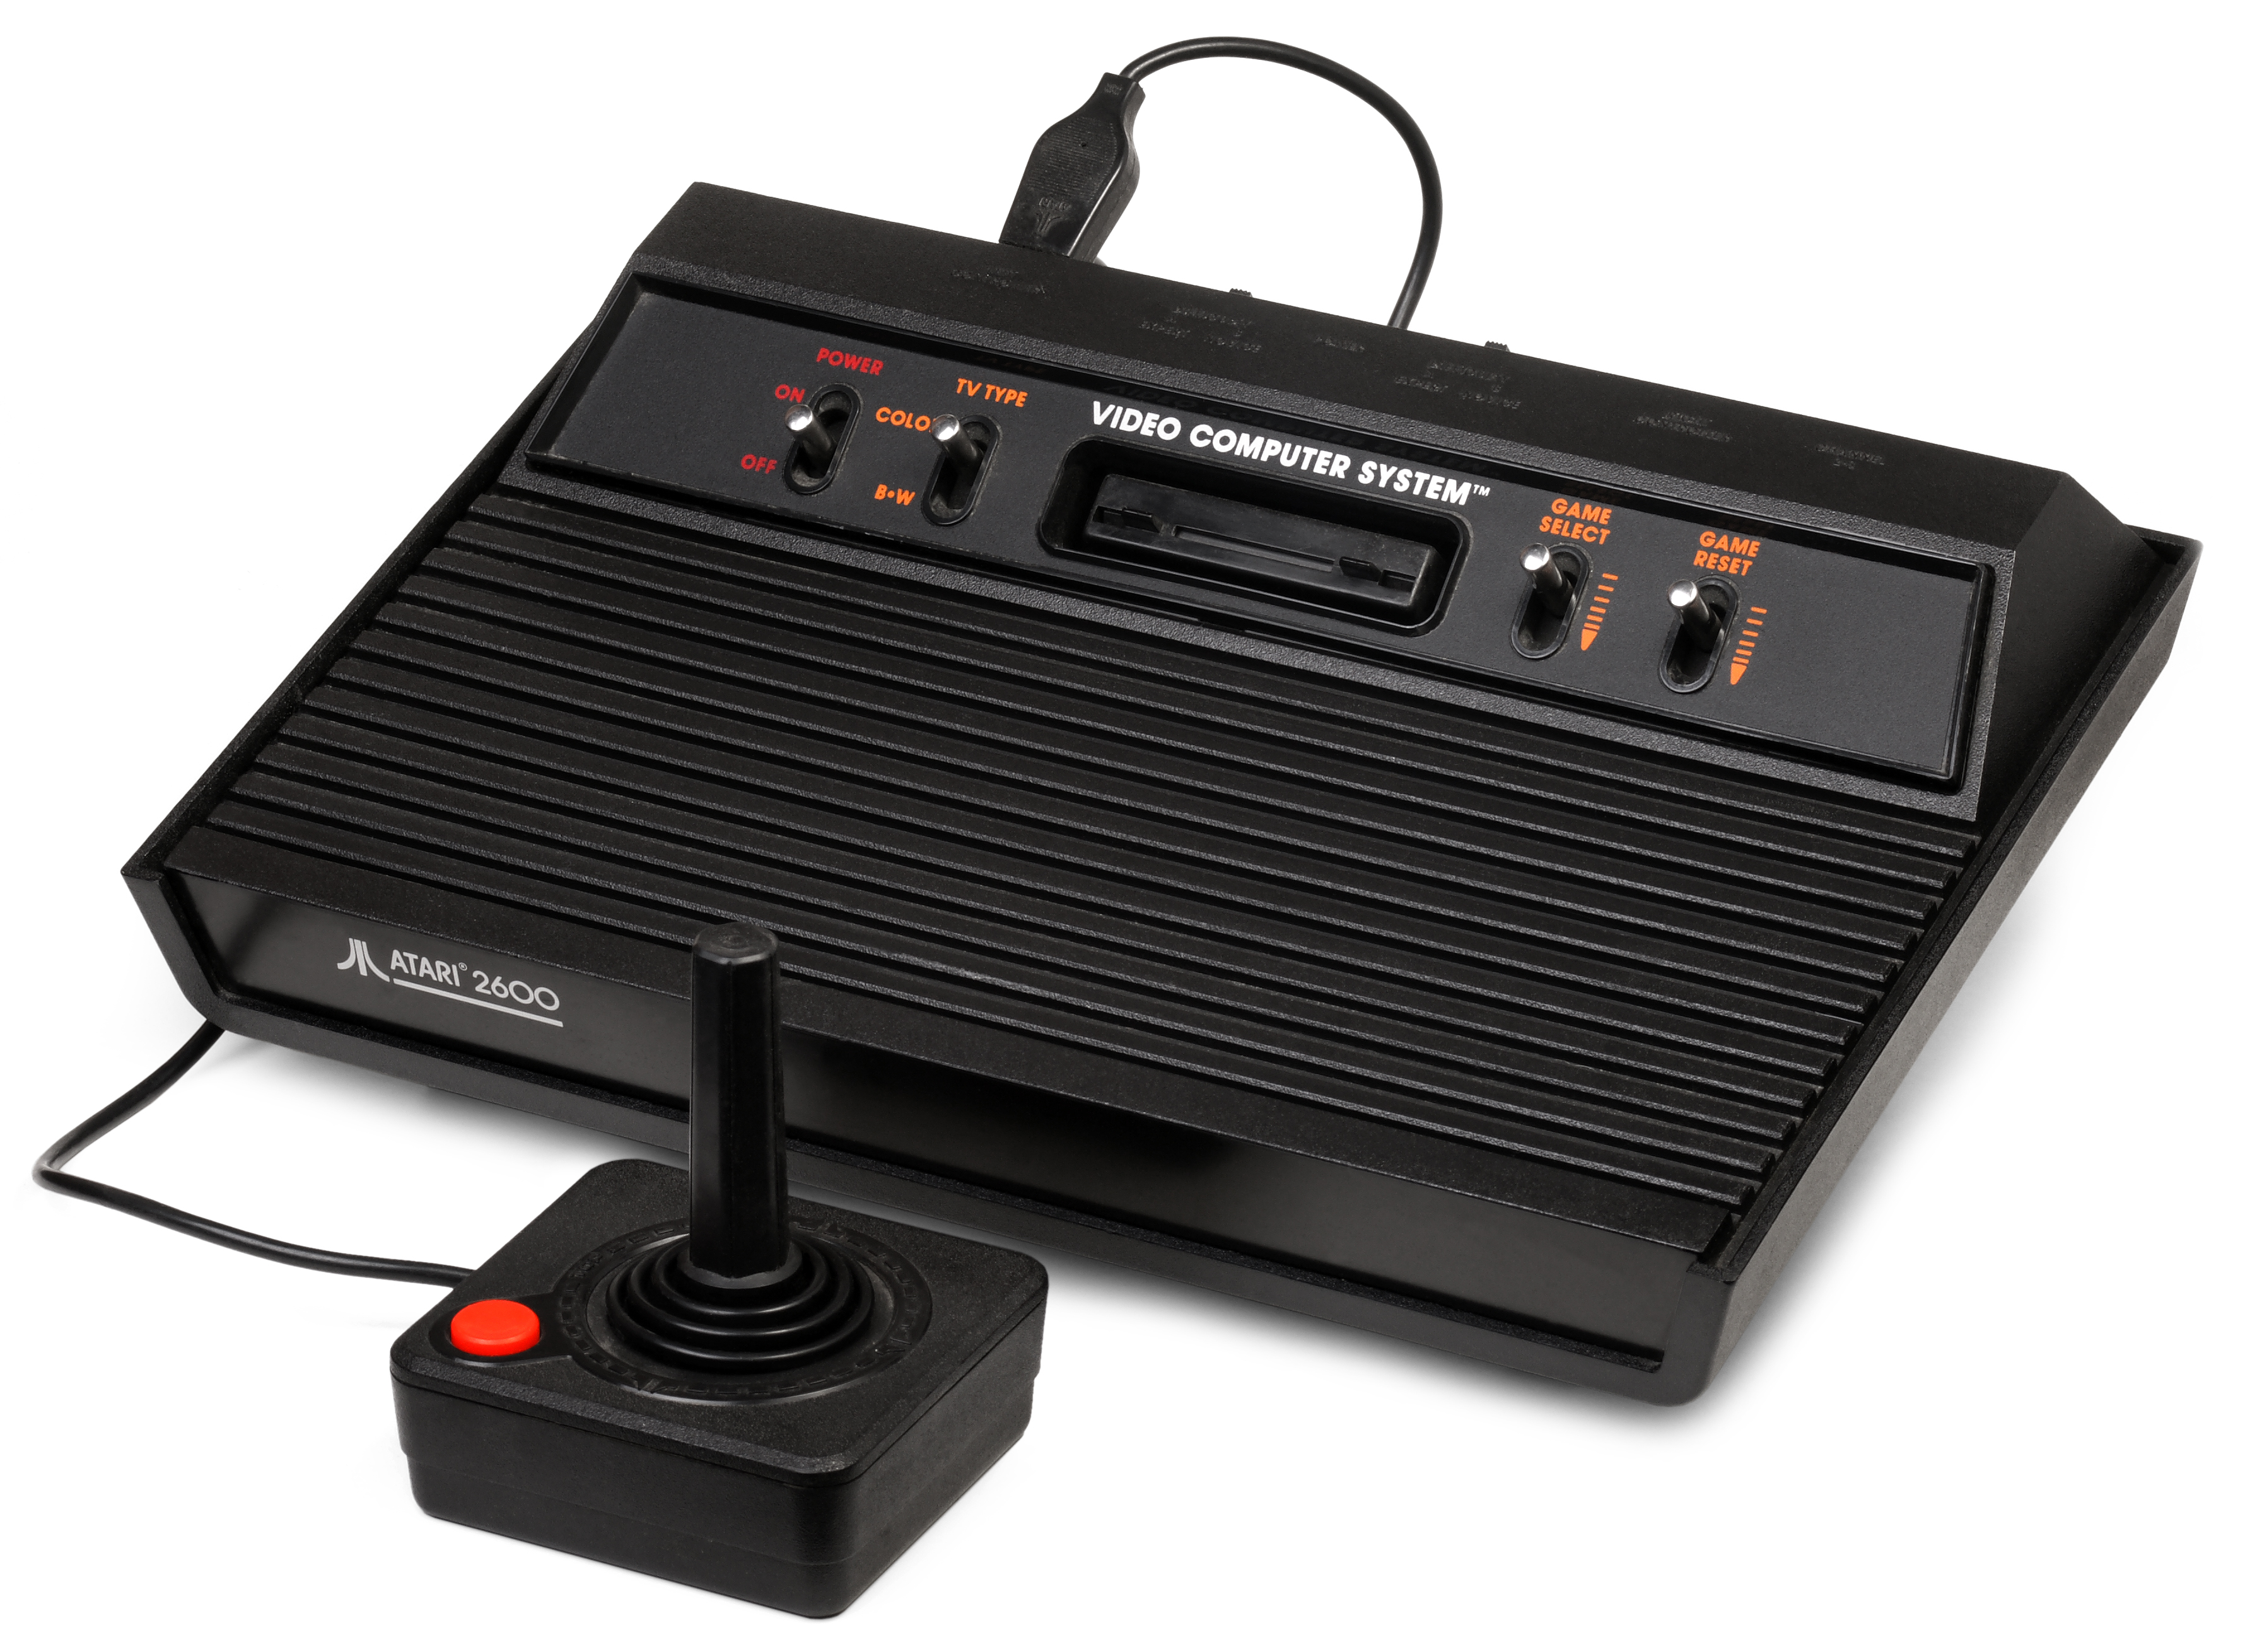
\includegraphics[width=90mm]{Atari2600Console.jpg}
	\caption{Hệ máy chơi game Atari 2600}
	\label{fig:AtariConsole}
\end{figure}

\section{Các thiết lập thực nghiệm}
	Chúng em thực hiện huấn luyện hệ thống trên ba trò chơi: \textit{Assault}, \textit{Breakout} và \textit{Seaquest}.
	Việc thực nghiệm trên ba trò chơi là để chứng minh hướng tiếp cận kết hợp học sâu với học tăng cường có thể áp dụng vào nhiều trò chơi khác nhau.
	\textit{Assault} là trò chơi bắn máy bay truyền thống: hệ thống điều khiển máy bay bay qua trái, phải hoặc bắn tên lửa để hạ máy bay địch.
	\textit{Breakout} là trò chơi ``phá gạch'': hệ thống điều khiển một mái chèo (paddle) qua trái, phải để giữ cho trái banh không rơi xuống dưới; phía trên là những viên gạch bị phá huỷ và cho điểm thưởng khi chạm phải trái banh.
	Cuối cùng là trò chơi \textit{Seaquest} có nội dung tương tự như ``Assault'' nhưng là điểu khiển tàu ngầm theo cả tám hướng xung quanh.
	Tuy các trò chơi này có nội dung tương tự nhau nhưng luật chơi cụ thể lại rất khác biệt và đòi hỏi chiến thuật mang tính ``dài hơi''.
	Ví dụ như màn hình trò chơi \textit{Seaquest} có một thanh không khí thể hiện mức độ không khí còn lại trong tàu ngầm.
	Khi thanh này cạn thì ta cần điều khiển tàu ngầm nổi lên mặt nước để lấy không khí.
	Vì vậy, hệ thống cần học được đặc trưng thể hiện mức không khí còn lại và dựa vào đó để điều khiển tàu ngầm nổi lên mặt nước.
	Ngoài ra, để chơi tốt và đạt nhiều điểm, hệ thống cần học được chiến thuật đợi không khí còn lại ít nhất rồi mới nổi lên mặt nước một lần để tiết kiệm thời gian.
	Ví dụ này cho thấy các trò chơi này đều đòi hỏi các đặc trưng học được phải rất trừu tượng và chiến thuật chơi cũng phải khá phức tạp.
	Hình () thể hiện màn hình một khung ảnh của ba trò chơi trên.
	
	Để giảm bớt tính toán của mô hình, khung ảnh RGB đầu vào được chuyển về ảnh mức xám (grayscale) và được giảm kích thước về $84\times84$.
	Để lưu thông tin về sự di chuyển và tốc độ của các đối tượng trong ảnh, ta ghép bốn khung ảnh liên tiếp nhau lại thành một trạng thái.
	Vậy một trạng thái lúc này sẽ gồm bốn ảnh mức xám $84\times84$ và được đưa trực tiếp vào ``input'' của mạng nơ-ron.
	Ngoài ra, do các khung hình gần nhau thường không thay đổi nhiều, một kỹ thuật đơn giản để tăng tốc độ huấn luyện đó là ta lặp lại một hành động cho $k$ khung hình liên tiếp.
	Nhờ kỹ thuật này, ta có thể huấn luyện nhiều hơn $k$ lần so với khi không áp dụng.
	Trong thực nghiệm này, chúng em chọn $k$ bằng 4 theo đề xuất của (\cite{mnih2013playing}).
	
	Cấu trúc mạng nơ-ron tích chập được dùng để xấp xỉ hàm giá trị là ``Deep Q-Network'' (\cite{mnihdqn2015}).
	Mạng này bao gồm bốn tầng ẩn với ba tầng đầu là tầng tích chập và tầng cuối là tầng ``Fully-connected''.
	Tầng tích chập đầu tiên gồm $32$ bộ lọc với kích thước $8\times8$ và bước dịch chuyển (stride) là $4\times4$.
	Tầng tích chập thứ hai gồm $64$ bộ lọc với kích thước $4\times4$ và bước dịch chuyển là $2\times2$.
	Tầng tích chập cuối cùng gồm $64$ bộ lọc với kích thước $3\times3$ và bước dịch chuyển là $1\times1$.
	Đầu ra của tầng tích chập được đưa vào một tầng ``Fully-connected'' gồm $512$ nơ-ron ẩn để tổng hợp đặc trưng.
	Tầng ``output'' của mạng cũng là một tầng ``Fully-connected'' với số nơ-ron ẩn là số hành động của trò chơi (6 cho ``Assault'', 4 cho ``Breakout'' và 18 cho ``Seaquest'').
	Tầng này sẽ trả về giá trị hành động tương ứng cho trạng thái đầu vào.
	Hàm kích hoạt của tất cả các tầng ẩn là hàm ``Rectified'': $\sigma(x) = \max(0, x)$.
	
	Để huấn luyện mạng nơ-ron này, chúng em áp dụng thuật toán ``RMSprop'' (\cite{tieleman2012lecture}) để tối tiểu hàm lỗi bình phương.
	Đây là một thuật toán cải tiến của SGD với ý tưởng chọn một hệ số học khác nhau cho từng trọng số của mạng nơ-ron.
	Hệ số học của mỗi trọng số sẽ phụ thuộc vào giá trị đạo hàm của hàm lỗi đối với trọng số này ở các bước cập nhật trước.
	Cụ thể hơn, nếu trọng số này được cập nhật ít ở những lần cập nhật trước thì hệ số học sẽ được tăng lên; trọng số được cập nhật nhiều thì sẽ có hệ số học giảm đi.
	Nhờ thuật toán này mà mức độ thay đổi của các trọng số là tương đương nhau.
	
	Chúng em sử dụng ``Python'' (kết hợp với framework ``Theano'' (\cite{2016arXiv160502688short})) làm ngôn ngữ lập trình chính.
	Do việc huấn luyện đòi hỏi sức mạnh tính toán rất lớn nên chúng em thực hiện cài đặt tính toán song song trên GPU để tăng tốc.
	GPU được dùng là NVIDIA GTX 980.
	
	Với các thiết lập thực nghiệm trên, chúng em tiến hành huấn luyện ba trò chơi với hai thuật toán ``Q-learning'' và ``Double Q-learning''.
	Mỗi trò chơi với mỗi thuật toán được huấn luyện $50$ triệu hành động.
	Thời gian huấn luyện là khoảng 50 giờ cho mỗi trò chơi với mỗi thuật toán.
	
\section{Thuật toán ``Q-learning''}
	Để thực nghiệm khả năng học và tự động chơi game, chúng em thực hiện thử nghiệm thuật toán ``Q-learning'' kết hợp với học sâu.
	Chúng em sử dụng chính sách $\epsilon$-greedy để làm chính sách khám phá không gian trạng thái và không gian hành động.
	$\epsilon$-greedy được chọn ở đây là vì chính sách này đơn giản cho việc cài đặt mà vẫn đảm bảo khả năng khám phá không gian cũng như khai thác kiến thức đã học của mô hình.
	Do ban đầu hệ thống chưa có nhiều hiểu biết về môi trường, chúng ta nên khám phá nhiều hơn; sau khi có một số hiểu biết nhất định thì hệ thống lại cần khai thác những hiểu biết đó.
	Ý tưởng này có thể dễ dàng được cài đặt bằng cách giảm dần hệ số $\epsilon$ trong khi đang huấn luyện.
	Với thuật toán ``Q-learning'', chúng em thực hiện giảm dần $\epsilon$ từ $1.0$ về $0.1$ trong $1$ triệu hành động đầu tiên.
	
	Để tiện cho việc quan sát kết quả và thử nghiệm hệ thống, chúng em chia quá trình huấn luyện $50$ triệu hành động ra thành $200$ ``epoch'' (tức mỗi ``epoch'' bao gồm $250000$ hành động).
	Sau mỗi ``epoch'', chúng em kiểm thử bộ trọng số học được trên $30$ màn chơi và lưu lại điểm số trung bình.
	Kết quả điểm số cuối cùng được báo cáo của mỗi trò chơi là giá trị điểm số lớn nhất của $200$ epoch.
	Các thiết lập trên tương đồng với (\cite{mnihdqn2015}) để việc so sánh là công bằng nhất.
	
	Một đặc điểm của bài toán tự động chơi game đó là kết quả điểm thưởng sau từng ``epoch'' thường rất nhiễu.
	Giá trị của các trọng số mạng nơ-ron có thể thay đổi ít sau mỗi ``epoch'' nhưng hàm giá trị tương ứng sẽ thay đổi nhiều.
	Điều này dẫn đến chính sách tương ứng cũng thay đổi nhiều làm cho điểm thưởng nhận được khi chơi game của các chính sách này sẽ rất khác nhau.
	Vì vậy nếu ta chỉ quan sát đồ thị điểm thưởng của quá trình kiểm thử sau mỗi ``epoch'', ta sẽ không biết chắc là hệ thống có đang chơi tốt lên hơn không.
	Một cách khác để quan sát quá trình học được đề xuất bởi (\cite{mnih2013playing}) đó là ta quan sát đồ thị giá trị của một tập trạng thái sau từng ``epoch''.
	Đầu tiên, ta thực hiện chơi game một cách ngẫu nhiên và lưu lại một tập các trạng thái gặp được trong quá trình chơi này (gọi là tập ``hold-out'').
	Trong quá trình huấn luyện, sau mỗi ``epoch'', ta tính trung bình giá trị hành động tốt nhất của các trạng thái trong tập ``hold-out''.
	Một chính sách chơi tốt thì thường sẽ đánh giá các hành động của các trạng thái trong tập ``hold-out'' cao hơn so với các chính sách chơi không tốt.
	Vì vậy, quan sát đồ thị này là một cách đơn giản để theo dõi quá trình học của hệ thống.
	\begin{figure}
		\centering
		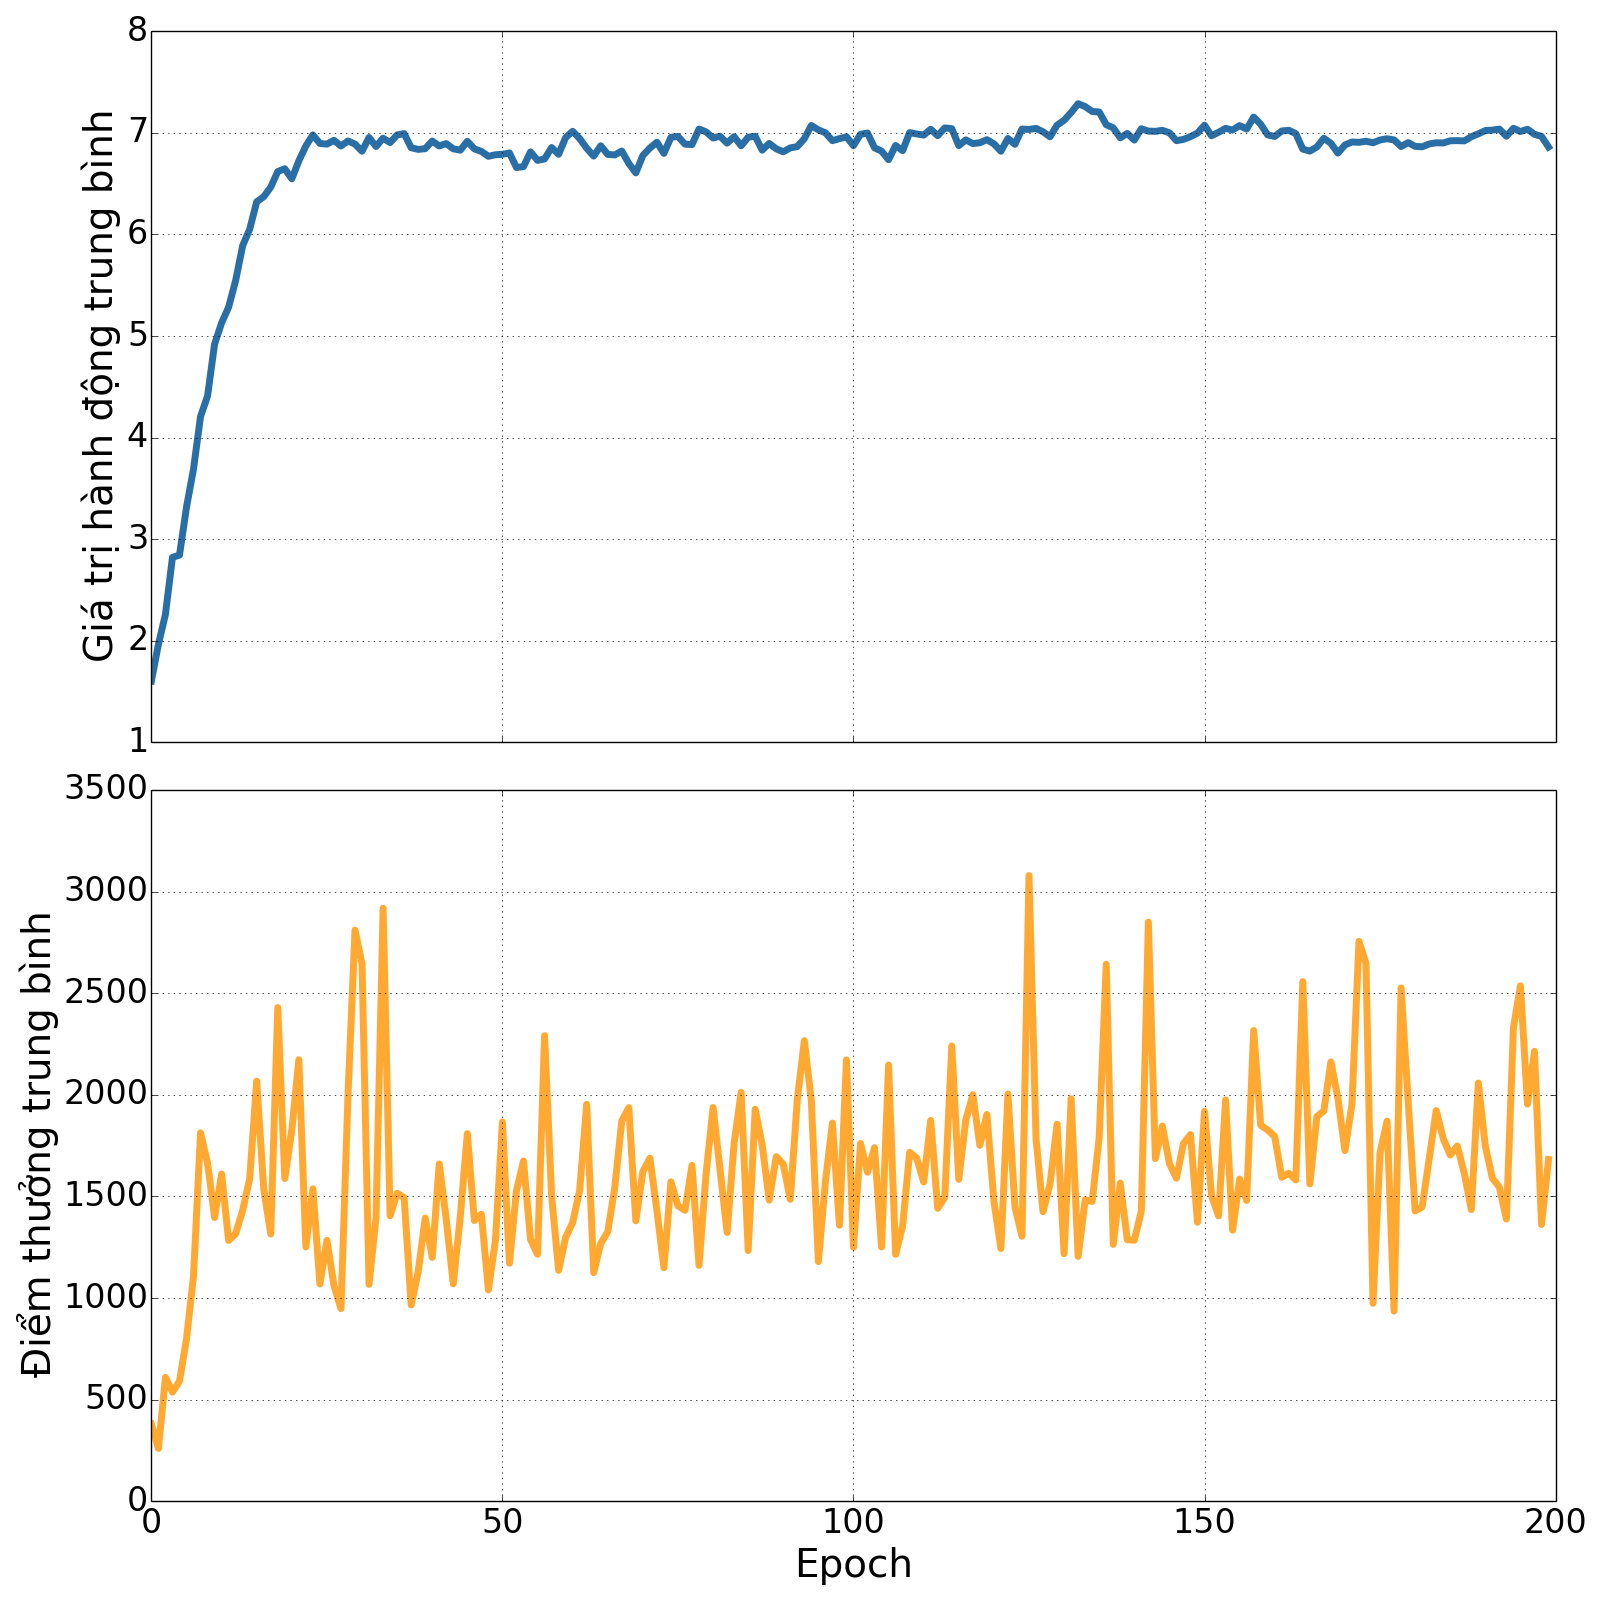
\includegraphics[width=\textwidth]{dqn_assault_values_rewards}
		\caption[Đồ thị giá trị hành động trung bình và điểm thưởng trung bình]{
		Đồ thị kết quả của trò chơi \textit{Assault}. 
		Đồ thị ở trên thể hiện trung bình giá trị hành động trên tập ``hold-out'' theo ``epoch'' huấn luyện; đồ thị ở dưới thể hiện điểm thưởng trung bình theo ``epoch'' huấn luyện.
		Điểm thưởng trung bình thay đổi rất nhiều sau từng ``epoch''.
		Nếu sử dụng đồ thị này để theo dõi quá trình huấn luyện thì ta sẽ không biết là hệ thống có đang học được cách chơi game hay không.
		Trong khi đó, đồ thị giá trị hành động lại ít nhiễu hơn và hội tụ dần đến một mức nhất định.
		Quan sát đồ thị này, ta thấy những ``epoch'' đầu hệ thống học rất nhanh và sau khoảng $50$ ``epoch'' thì giá trị hành động không tăng cao hơn nữa.
		Lúc này, ta có thể dừng việc học sớm.
		Tuy nhiên, một số game có thể cần học lâu hơn.
		Vì vậy, chúng em cố định số ``epoch'' để huấn luyện được nhiều trò chơi mà không phải thay đổi siêu tham số.}
		\label{fig_assault_vr}
	\end{figure}
	
	Hình (\ref{fig_assault_vr}) thể hiện đồ thị điểm số và giá trị trạng thái trên tập ``hold-out'' của trò chơi \textit{Assault}.
	Điểm thưởng kết quả của ba game được báo cáo trong bảng (\ref{table_dqn_results}).
	Cả ba game được thực nghiệm cho kết quả vượt xa kết quả chơi ngẫu nhiên.
	Điều này cho thấy hệ thống thật sự học được cách chơi để đạt được nhiều điểm số dù ban đầu không hề biết quy luật chơi.
	Hai trong số ba game còn cho kết quả hơn cả kết quả do con người chơi.
	Tuy nhiên, bài báo \cite{mnihdqn2015} chỉ cho người chơi học thử khoảng 2 giờ cho mỗi game, ít hơn nhiều so với việc huấn luyện $50$ triệu hành động (tức khoảng 38 ngày chơi) của hệ thống.
	Vì vậy, điểm thưởng nhận được của con người trong bảng (\ref{table_dqn_results}) chỉ mang tính tham khảo.
	Dù chúng em thực hiện cài đặt lại thuật toán được đề xuất bởi bài báo \cite{mnihdqn2015} nhưng kết quả cũng không bằng nhau (cao hơn ở game \textit{Seaquest} và thấp hơn ở hai game còn lại).
	Lý do chính của điều này là vì cách cài đặt khác nhau và chương trình giả lập game Atari khác nhau.
	
	\begin{table}
		\centering
		\caption[Điểm thưởng nhận được của thuật toán ``Q-learning'']{
		Kết quả \textit{Ngẫu nhiên} nhận được bằng cách chơi với chính sách ngẫu nhiên (chọn hành động theo phân bố đều).
		Kết quả \textit{Con người} nhận được bằng cách cho một số người học và chơi các game này.
		\textit{Kết quả gốc} là kết quả thực nghiệm của bài báo \cite{mnihdqn2015}.
		Kết quả \textit{Thực nghiệm} là kết quả do nhóm thực hiện cài đặt lại thuật toán ``Q-learning''.
		Giá trị được in đậm là giá trị lớn nhất của mỗi dòng.}
		\label{table_dqn_results}
		\begin{tabular}{| l | c | c | c | c |}
			\hline
			 & \textit{Ngẫu nhiên}\cite{mnihdqn2015} & \textit{Con người}\cite{mnihdqn2015} & \textit{Kết quả gốc}\cite{mnihdqn2015} & \textit{Thực nghiệm} \\
			\hline \hline
			\textit{Assault} & 222.4 & 742.0 & \textbf{4,280.4} & 3,078.8 \\ 
			\hline
			\textit{Breakout} & 1.7 & 30.5 & \textbf{385.5} & 377.6 \\ 
			\hline
			\textit{Seaquest} & 68.4 & \textbf{42,054.7} & 5,860.6 & 6,340.7 \\ 
			\hline
		\end{tabular}		
	\end{table}

\section{Thuật toán ``Double Q-learning''}
	Chúng em thực hiện cài đặt và thử nghiệm lại thuật toán ``Double Q-learning'' \cite{hasselt2010double}, \cite{van2015deep} để giải quyết vấn đề đánh giá quá cao.
	Các thiết lập thực nghiệm đều giống như khi thực nghiệm thuật toán ``Q-learning''.
	Tuy nhiên, để tương đồng với cài đặt của bài báo \cite{van2015deep}, chúng em giảm hệ số $\epsilon$ từ $1.0$ xuống $0.01$ (thay vì $0.1$ như ở phần thực nghiệm ``Q-learning'') trong $1$ triệu hành động đầu tiên của quá trình huấn luyện.
	
	\begin{table}
		\centering
		\caption[Điểm thưởng nhận được của thuật toán ``Double Q-learning'']{
		Kết quả \textit{Ngẫu nhiên} và \textit{Con người} được trích từ bài báo \cite{van2015deep}.
		Do môi trường giả lập game khác nhau nên chúng em chỉ so sánh ``Double Q-learning'' với phiên bản cài đặt ``Q-learning'' của nhóm thay vì so sánh với phiên bản ``Double Q-learning'' của bài báo \cite{van2015deep}.
		Giá trị được in đậm là giá trị lớn nhất của mỗi dòng.}
		\label{table_double_results}
		\begin{tabular}{| l | c | c | c | c |}
			\hline
			 & \textit{Ngẫu nhiên}\cite{mnihdqn2015} & \textit{Con người}\cite{mnihdqn2015} & \textit{Q-learning} & \textit{Double Q-learning} \\
			\hline \hline
			\textit{Assault} & 222.4 & 742.0 & 3,078.8 & \textbf{4864.6} \\
			\hline
			\textit{Breakout} & 1.7 & 30.5 & 377.6 & \textbf{431.2} \\
			\hline
			\textit{Seaquest} & 68.4 & \textbf{42,054.7} & 6,340.7 & 13,186 \\
			\hline
		\end{tabular}		
	\end{table}
	
	Bảng \ref{table_double_results} cho biết kết quả của thuật toán ``Double Q-learning'' trên ba game.
	Thuật toán ``Double Q-learning'' cho kết quả tốt hơn hẳn điểm số của ``Q-learning'' trên cả ba game và cao hơn gấp đôi ở game \textit{Seaquest}.
	Lý do ``Double Q-learning'' hoạt động tốt như vậy trên game \textit{Seaquest} là vì game này có nhiều hành động (18 so với 4 của \textit{Breakout} và 6 của \textit{Assault}).
	Số lượng hành động càng nhiều thì khả năng bị đánh giá quá cao lại càng tăng.
	Vì vậy, thuật toán ``Q-learning'' bị ảnh hưởng rất lớn bởi vấn đề đánh giá quá cao và thuật toán ``Double Q-learning'' cho kết quả tốt hơn hẳn khi giải quyết được vấn đề này.
	Các kết quả này cho thấy thuật toán ``Double Q-learning'' là một cải tiến rất tốt cho bài toán tự động chơi game.
	
	Để thấy rõ hơn việc hạn chế vấn đề đánh giá quá cao của ``Double Q-learning'', ta có thể coi đồ thị giá trị hành động trung bình trên tập ``hold-out'' và đồ thị điểm thưởng trung bình của cả hai thuật toán ở hình (\ref{fig_double_compare}).
	Thuật toán ``Double Q-learning'' cho kết quả điểm thưởng tốt hơn hẳn ``Q-learning'' vì đánh giá hành động chính xác hơn (không bị vấn đề đánh giá quá cao).
	
	\begin{figure}
		\centering
		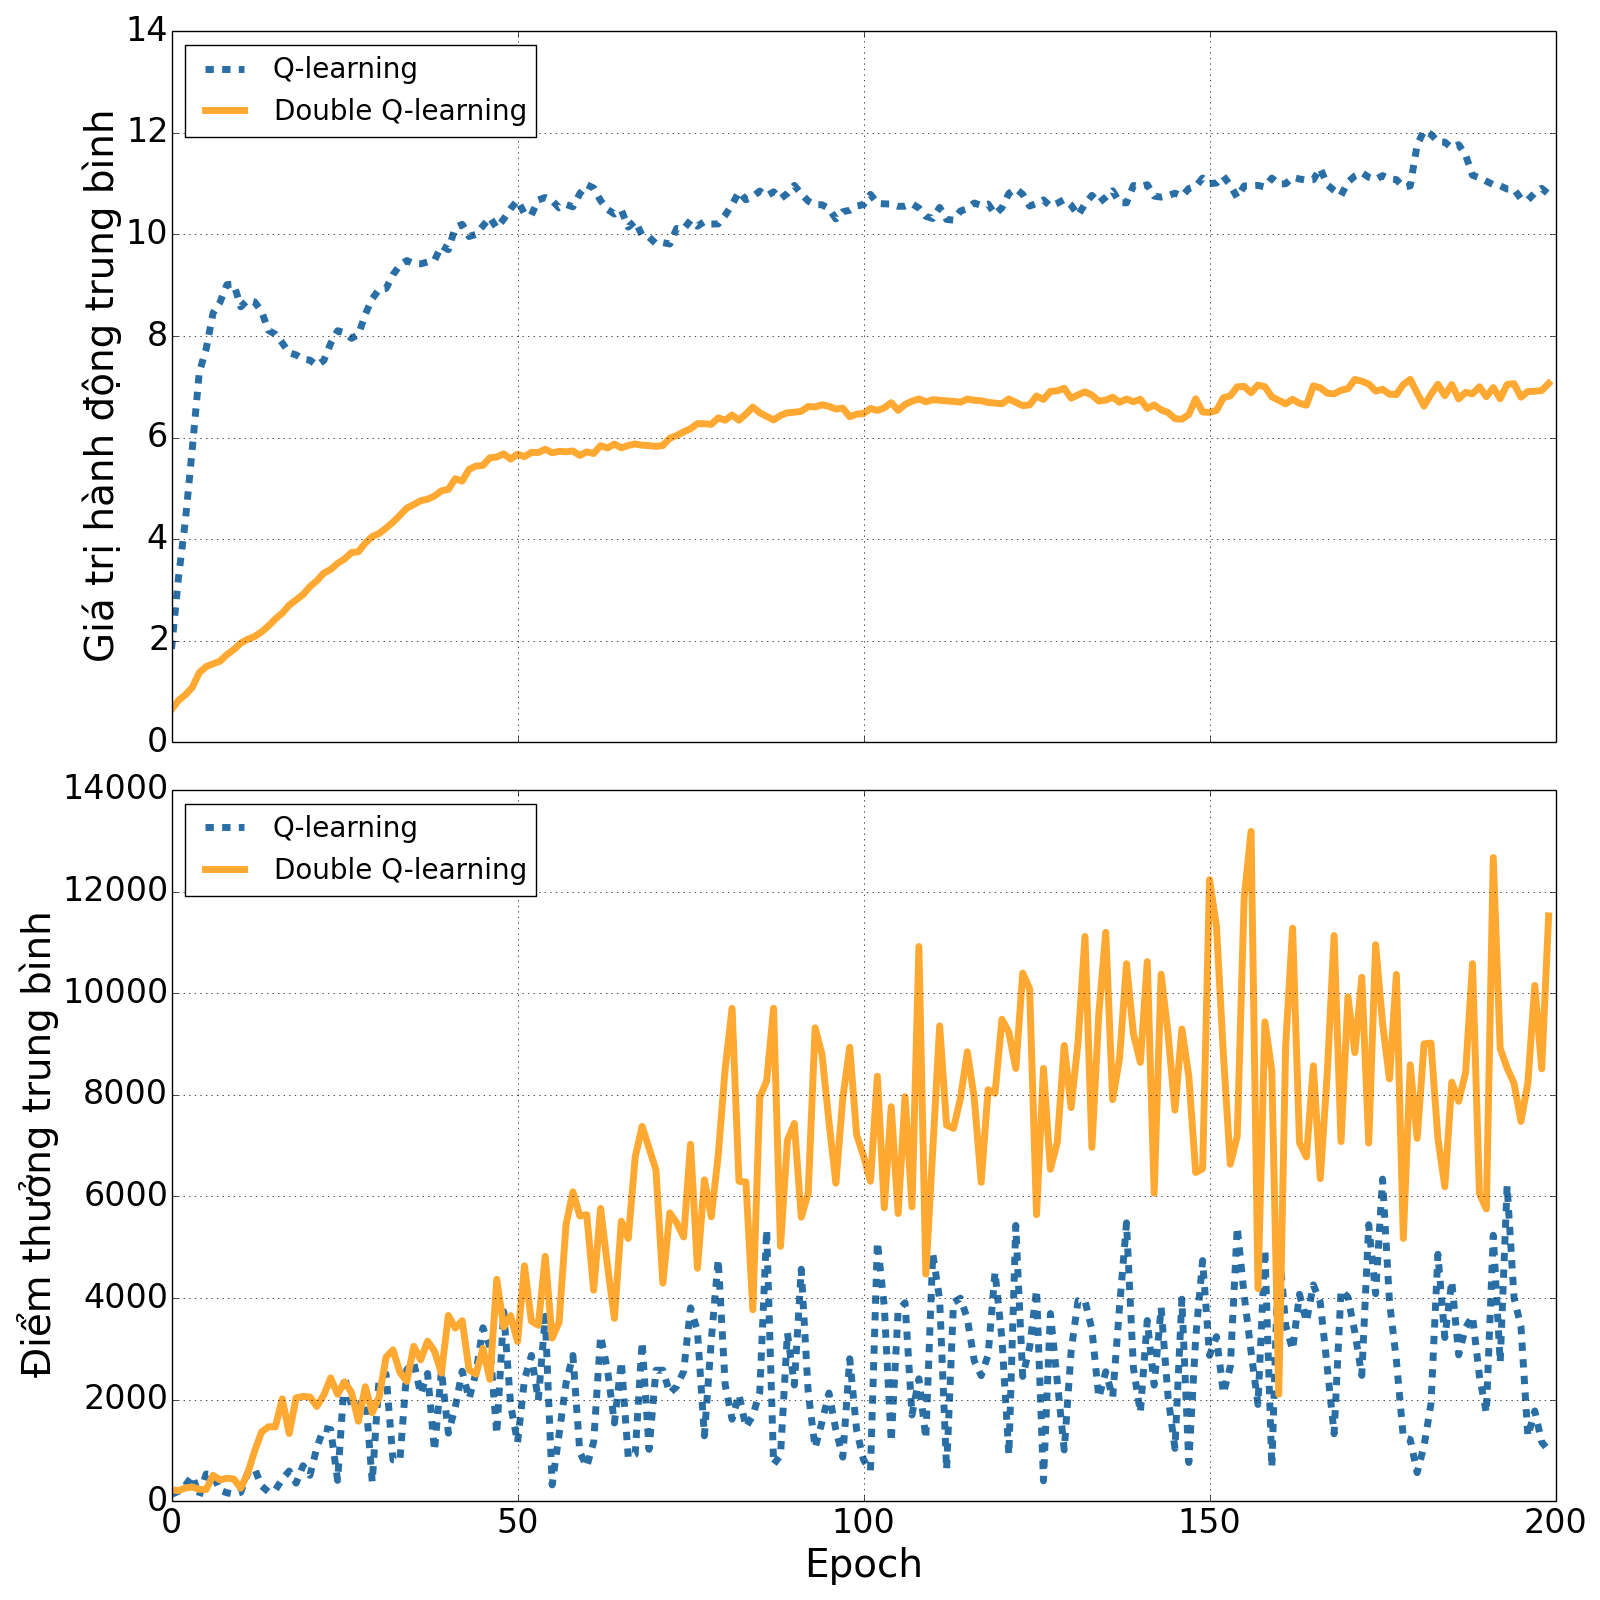
\includegraphics[width=\textwidth]{double_compare}
		\caption[Đồ thị giá trị hành động trung bình và điểm thưởng trung bình của hai thuật toán]{
		Đồ thị kết quả của trò chơi \textit{Seaquest}.
		Hình phía trên là đồ thị giá trị hành động trung bình theo ``epoch''; hình phía dưới là đồ thị điểm thưởng trung bình theo ``epoch''.
		Ở đồ thị phía trên, thuật toán ``Q-learning'' đánh giá rất cao các hành động của trạng thái thuộc tập ``hold-out''.
		Tuy nhiên, khi chơi thử game thì thuật toán ``Q-learning'' lại cho điểm thưởng rất thấp.
		Điều này cho thấy thuật toán ``Q-learning'' gặp vấn đề đánh giá quá cao và vấn đề này ảnh hưởng đến kết quả chơi game của hệ thống.
		Trong khi đó, thuật toán ``Double Q-learning'' tuy đánh giá các hành động của trạng thái thuộc tập ``hold-out'' thấp hơn nhưng khi chơi game thì lại được nhiều điểm thưởng hơn.
		Thuật toán ``Double Q-learning'' đánh giá chính xác hơn giá trị hành động và vì thế, chính sách chơi game cũng tốt hơn.}
		\label{fig_double_compare}
	\end{figure}
		
\section{Phân tích hàm giá trị hành động}
	Để thấy rõ hơn khả năng xấp xỉ hàm giá trị của mạng nơ-ron, ta có thể xem xét giá trị của một số trạng thái trong quá trình chơi game.
	Cụ thể hơn, chúng em thực hiện lưu một số ``frame'' ảnh trong quá trình chơi cùng với giá trị của chúng được tính từ mạng nơ-ron (với thuật toán ``Q-learning'').
	
	Hình \ref{seaquest:frames} và đồ thị \ref{fig_seaquest_frames} thể hiện các ``frame'' ảnh và giá trị của các trạng thái tương ứng.
	Quan sát giá trị tương đối của các trạng thái liên tiếp nhau trong một lần chơi, ta có thể thấy mạng nơ-ron học được một hàm giá trị phức tạp và có ý nghĩa cao.
	Nhờ hàm giá trị được xấp xỉ tốt, chính sách chơi game mới lựa chọn hành động hợp lý để nhận được điểm thưởng cao nhất có thể.
	
	\begin{figure}
		\begin{subfigure}{.5\textwidth}
			\centering
			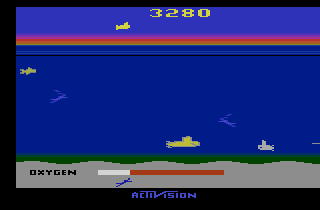
\includegraphics[width=.8\linewidth]{008182}
			\caption{}
			\label{seaquest:frame_1}
		\end{subfigure}%
		\begin{subfigure}{.5\textwidth}
			\centering
			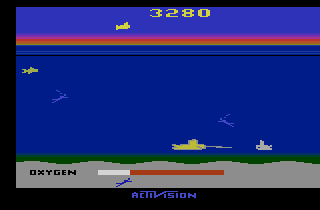
\includegraphics[width=.8\linewidth]{008185}
			\caption{}
			\label{seaquest:frame_2}
		\end{subfigure}\\[2ex]
		\begin{subfigure}{.5\textwidth}
			\centering
			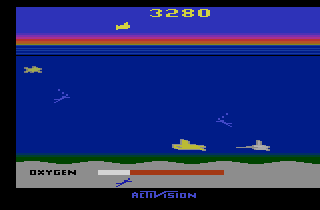
\includegraphics[width=.8\linewidth]{008188}
			\caption{}
			\label{seaquest:frame_3}
		\end{subfigure}%
		\begin{subfigure}{.5\textwidth}
			\centering
			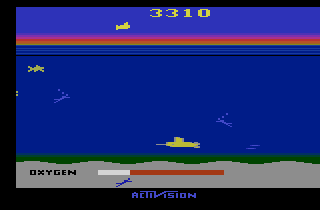
\includegraphics[width=.8\linewidth]{008191}
			\caption{}
			\label{seaquest:frame_4}
		\end{subfigure}%
		\caption[Hình ảnh một số ``frame'' của trò chơi \textit{Seaquest}]{Hình ảnh 4 ``frame'' của trò chơi \textit{Seaquest}.
		Ở ``frame'' đầu tiên (hình \ref{seaquest:frame_1}), tàu ngầm do hệ thống điều khiển ở giữa và tàu ngầm địch ở bên phải.
		Ở ``frame'' kế tiếp (hình \ref{seaquest:frame_2}), hệ thống thực hiện hành động phóng ngư lôi.
		Tiếp đó (hình \ref{seaquest:frame_3}), ngư lôi trúng tàu ngầm địch.
		Cuối cùng (hình \ref{seaquest:frame_4}), tàu ngầm địch bị phá huỷ cho điểm thưởng.
		Các ``frame'' này ứng với các giá trị trong đồ thị ở hình \ref{fig_seaquest_frames}.}
		\label{seaquest:frames}
	\end{figure}
	
	\begin{figure}
		\centering
		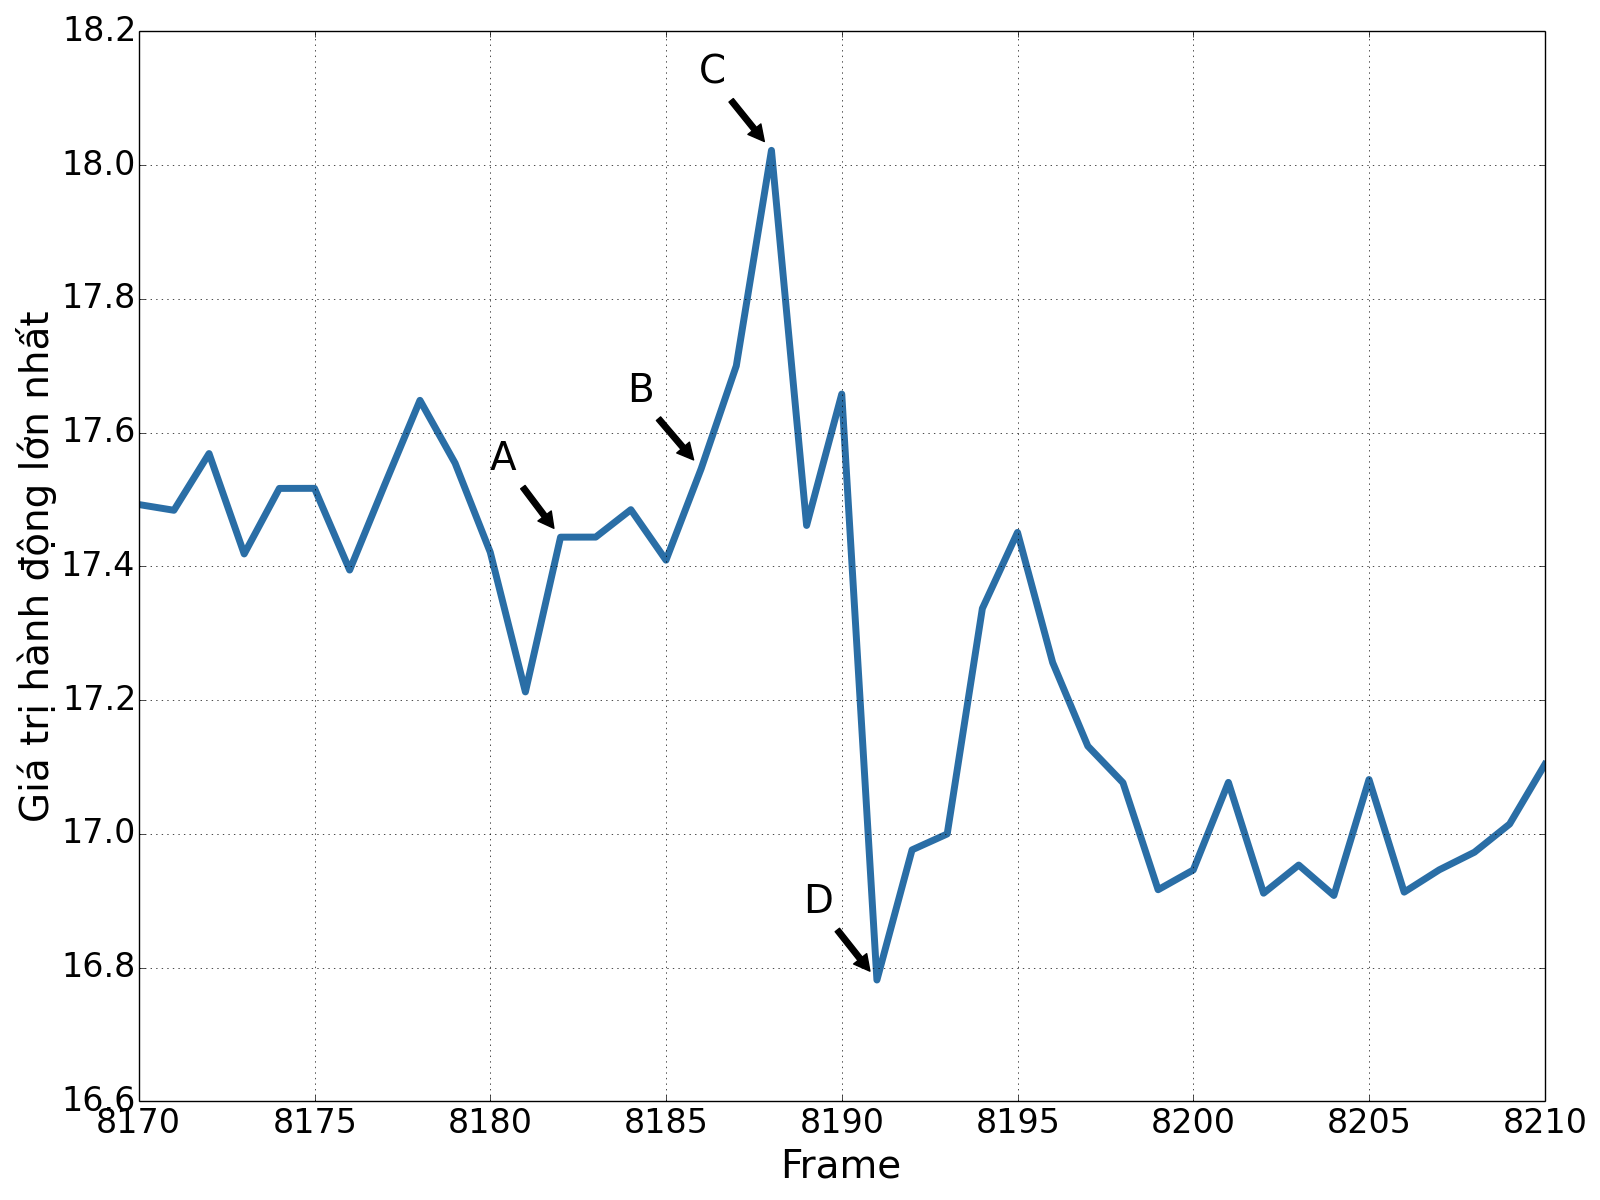
\includegraphics[width=\textwidth]{dqn_seaquest_frames}
		\caption[Đồ thị giá trị hành động của một số trạng thái trong một lần chơi game]{
		Đồ thị thể hiện giá trị hành động lớn nhất tại một số trạng thái; các trạng thái này ứng với các ``frame'' trò chơi \textit{Seaquest}.
		Tại ``frame'' được đánh dấu \textit{A}, giá trị hành động lớn nhất đang ở mức trung bình ứng với việc tàu ngầm của ta chưa thực hiện hành động gì ảnh hưởng đến điểm số.
		Tại ``frame'' \textit{B}, tàu ngầm của ta bắn ngư lôi về phía tàu ngầm địch.
		Mạng nơ-ron khi nhận được ``frame'' ảnh này ``hiểu'' được rằng nếu ngư lôi chạm vào địch thì ta sẽ nhận được điểm thưởng.
		Vì vậy, đồ thị giá trị bắt đầu tăng lên đến ''frame'' \textit{C}.
		Tại ``frame'' \textit{C}, ngư lôi trúng tàu ngầm địch nên việc nhận được điểm là chắc chắn; hàm giá trị biết được điều này nên đồ thị giá trị đạt đỉnh điểm tại đây.
		Sau khi nhận được điểm thưởng và tàu ngầm địch bị phá huỷ, mạng nơ-ron nhận thấy rằng xung quanh không có yếu tố nào có thể giúp tăng điểm số nên đánh giá ``frame'' \textit{D} có giá trị thấp.		
		}
		\label{fig_seaquest_frames}
	\end{figure}
